\section{Knowledge Gap Analysis and Evaluation}
% \section{Use Cases and Evaluation}

% This section will discuss use cases and evaluation of the research. The data used were taken from Wikidata and retrieved using Wikidata Query Service on March 2nd 2025.

In this section, we present the analysis and evaluation of knowledge gaps using real-world use cases. The analyses focus on identifying disparities in knowledge representation. All data were obtained from Wikidata via the Wikidata Query Service, retrieved on March 2nd, 2025.

% to be added:
% - data di-retrive kapan: [input date]
% - only consider truthy/direct property
% - cara akses data dari Wikidata, flow pemrosesan data (dengan diagram)

% \subsection{Bias in Wikidata}
\subsection{Group-Level Gap in Representation in Wikidata}

In this subchapter, analysis is conducted to see whether any particular entity group in Wikidata is underrepresented compared to others. There are 2 analysis done: gender-based gap and regional gap.


\paragraph{Gender Bias in Wikidata}
Gender bias analysis in Wikidata will be performed on 10 Wikidata classes: computer scientist, American singer, American actress/actor, badminton player, businessperson, lawyer, American politician, American writer, American researcher, and American journalist.

To analyze the bias, the first aspect that will be considered is the proportion of each gender in every class. We assume that there are equal numbers of males and females in real-world and this will be the basis to determine if there is any bias in the data. Pearson's chi-square test (goodness-of-fit) is then performed to test the null and alternative hypotheses with significance level of \(\alpha=5\%\) as follows:

\(H_0\): The proportions of males and females in a particular class are equal to the real-world proportion

\(H_1\): The proportions of males and females in a particular class are not equal to the real-world proportion

From \autoref{tab:gender - entity count}, we can see that there are more male entities than female entities in all of the classes. In terms of entity count, the gender gaps in some classes such as American singer, American actress/actor, badminton player, and American writer, are slim. The gender gaps in some other classes are huge, and it can be observed in the classes of computer scientist, businessperson, lawyer, American politician, journalist, and researcher. This phenomenon can also be easily identified through visualization, as exhibited in \autoref{fig:bias histogram-computer scientist}, where the histogram of the female subclass is much smaller compared to the male. Looking at the chi-square test result, as p-value is well below the chosen significance level, the null hypothesis is rejected in all classes. Hence, we consider the difference of entity count to be significant and conclude that the proportions of males and females in each Wikidata class are not the same as the assumed real-world proportion of 50\%-50\%.

However, it is arguable that, for some classes, the gap in entity count between both genders is expected because, in reality, there are more men than women in the workforce, especially in particular fields such as engineering. As a consequence, it is not reasonable if we expect to have an equal number of males and females entities in Wikidata. Therefore, entity count may not be a good measure of bias because of the nature of the data itself. To address this, we need to evaluate other metrics which can quantify the bias on entity-level.

\begin{center}
\small
\begin{threeparttable}
\caption{Entity Count of 10 Wikidata Classes per Gender Category}
\label{tab:gender - entity count}
\begin{tabular}{c | c c c c c c c} 

\toprule
    Class Name & Entity & Male & Female & \%Male & \%Female & $\chi^2$ & p-value \\ [0.5ex] 

\midrule
    American actress/actor & 38087 & 21451 & 16636 & 0.56 & 0.44 & 608.72 & 2.13e-134 \\
    American journalist & 17740 & 12223 & 5517 & 0.69 & 0.31 & 2534.97 & 0.0 \\
    American politician & 92901 & 83007 & 9894 & 0.89 & 0.11 & 57539.86 & 0.0 \\
    American researcher & 4867 & 3387 & 1480 & 0.70 & 0.30 & 747.21 & 1.63e-164 \\
    American singer & 15712 & 9027 & 6685 & 0.57 & 0.43 & 349.09 & 6.67e-78 \\
    American writer & 32573 & 19113 & 13460 & 0.59 & 0.41 & 981.07 & 2.34e-215 \\
    Computer scientist & 17914 & 15229 & 2685 & 0.85 & 0.15 & 8783.74 & 0.0 \\
    Badminton player & 25283 & 13377 & 11906 & 0.53 & 0.47 & 85.58 & 2.22e-20 \\
    Businessperson & 74538 & 66706 & 7832 & 0.89 & 0.11 & 46501.76 & 0.0 \\
    Lawyer & 91348 & 80639 & 10709 & 0.88 & 0.12 & 53533.79 & 0.0 \\ [1ex]
\bottomrule

\end{tabular}
\begin{tablenotes}
    \footnotesize
    \item{This table shows the entity count of 10 Wikidata classes per Gender Category. Chi-square test result shows the significance of difference between the entity count of the two genders male and female.}
\end{tablenotes}

\end{threeparttable}
\end{center}

The next metrics to be considered are the measures of central tendency and dispersion to see where the wealth distribution is concentrated and how the data spread.

From \autoref{tab:gender - central tendency}, female entities generally have lower values of measure of central tendency (mean, median, mode). These characteristics can also be observed from the histogram in \autoref{fig:bias histogram-computer scientist}: female histograms’ peak and dense area are located on the left of the male’s. The range of property count of females is generally also lower than males. However, there are some classes in which the richest entity is a female. An example for this is the class of American Singer, which is shown by \autoref{fig:bias histogram-american singer}. Though the value of mean, median, and mode of count of properties are lower for female compared to male, the richest entity on that class is a female entity Madonna (Q1744) with bag of property count of 687, with a significant difference with Michael Jackson (Q2831) with bag of property count of 574. We also observed positive values of skewness (skewness > 0) and high kurtosis values (kurtosis > 3) in all classes, denoting the wealth distribution is right skewed and leptokurtic.

\begin{center}
\small
\begin{threeparttable}
\caption{Measures of Central Tendency of 10 Wikidata Classes per Gender Category}
\label{tab:gender - central tendency}
\begin{tabular}{c | c c c} 

\toprule
    Class Name & \CellWithForceBreak{Mean \\ (o/m/f)} & \CellWithForceBreak{Median \\ (o/m/f)} & \CellWithForceBreak{Mode \\ (o/m/f)} \\ [0.5ex] 
\midrule
    American actress/actor & 38.96/39.85/37.80 & 29.00/30.00/28.00 & 19/19/22 \\
    American journalist & 30.71/32.44/26.89 & 23.00/25.00/20.00 & 14/14/14 \\
    American politician & 19.22/19.33/18.25 & 15.00/15.00/15.00 & 13/9/13 \\
    American researcher & 23.97/25.00/21.63 & 20.00/21.00/18.00 & 12/12/12 \\
    American singer & 42.78/42.99/42.51 & 31.00/33.00/30.00 & 18/24/15 \\
    American writer & 38.86/42.76/33.33 & 30.00/33.00/26.00 & 19/22/19 \\
    Computer scientist & 24.16/24.50/22.28 & 19.00/19.00/18.00 & 8/8/8 \\
    Badminton player & 21.50/21.25/21.78 & 16.00/16.00/16.00 & 13/13/13 \\
    Businessperson & 16.91/16.83/17.61 & 13.00/13.00/13.00 & 10/10/9 \\
    Lawyer & 22.44/22.98/18.37 & 19.00/19.00/15.00 & 16/16/12 \\
    [1ex]
\bottomrule
\end{tabular}
\begin{tablenotes}
    \footnotesize
    \item{This table shows the measures of central tendency of 10 Wikidata classes per gender category. Each measure will have 3 values: o (overall), m (male), and f (female).}
\end{tablenotes}
\end{threeparttable}
\end{center}


\begin{center}
\small
\begin{threeparttable}
\caption{Measures of Dispersion and Symmetry of 10 Wikidata Classes per Gender Category}
\label{tab:gender - dispersion and symmetry}
\begin{tabular}{c | c c c c c} 

\toprule
    Class Name & \CellWithForceBreak{Min \\ (o/m/f)} & \CellWithForceBreak{Max \\ (o/m/f)} & \CellWithForceBreak{Std. Deviation \\ (o/m/f)} & \CellWithForceBreak{Skewness \\ (o/m/f)} & \CellWithForceBreak{Kurtosis \\ (o/m/f)} \\ [0.5ex] 
\midrule
    American actress/actor & 4/4/4 & 687/574/687 & 33.89/32.75/35.28 & 4.23/3.54/4.94 & 30.74/21.59/39.53 \\
    American journalist & 4/5/4 & 402/402/353 & 26.84/28.14/23.23 & 4.21/4.18/4.15 & 30.73/30.18/29.38 \\
    American politician & 4/4/4 & 476/476/328 & 14.77/14.77/14.75 & 6.53/6.55/6.40 & 97.36/100.39/72.68 \\
    American researcher & 4/4/4 & 222/222/171 & 16.89/18.19/13.17 & 3.86/3.79/3.45 & 25.67/23.50/26.78 \\
    American singer & 4/4/4 & 687/574/687 & 39.35/35.33/44.21 & 4.09/3.16/4.61 & 29.38/18.24/33.19 \\
    American writer & 4/4/4 & 476/476/425 & 34.12/37.19/28.30 & 3.56/3.29/4.05 & 20.51/17.35/27.82 \\
    Computer scientist & 3/3/3 & 441/441/168 & 19.53/20.18/15.24 & 3.41/3.45/2.20 & 27.66/27.80/9.33 \\
    Badminton player & 4/9/4 & 360/238/360 & 16.09/15.28/16.96 & 4.23/3.89/4.48 & 30.85/22.98/35.97 \\
    Businessperson & 3/3/3 & 574/574/429 & 14.65/14.01/19.27 & 7.73/7.37/8.15 & 130.49/128.49/108.21 \\
    Lawyer & 3/3/3 & 550/550/328 & 16.61/16.91/13.47 & 5.56/5.59/5.23 & 76.02/76.31/64.39 \\[1ex]
\bottomrule
\end{tabular}
\begin{tablenotes}
    \footnotesize
    \item{This table shows the measures of dispersion and symmetry of 10 Wikidata classes per gender category. Each measure will have 3 values: o (overall), m (male), and f (female).}
\end{tablenotes}
\end{threeparttable}
\end{center}

\begin{figure}[htp]
\centering 
\subfloat[Histogram and Marginal Distribution Plot of Wealth for Class Computer Scientist\label{fig:bias histogram-computer scientist}]{%
  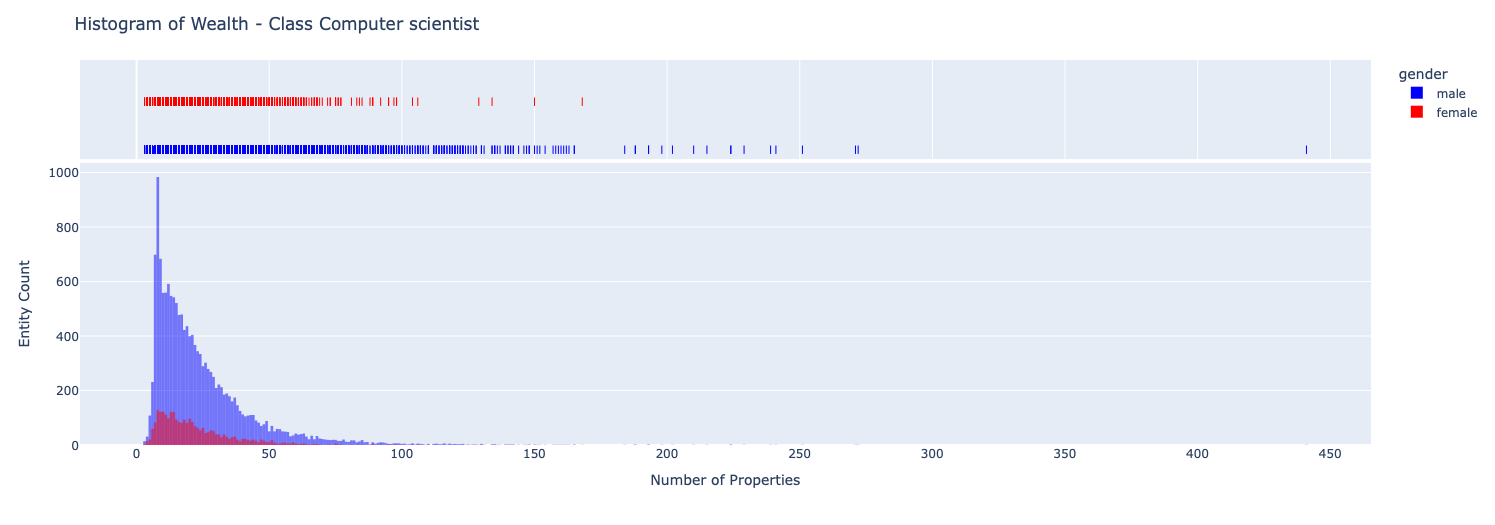
\includegraphics[clip,width=1.0\columnwidth]{Histogram of Wealth - Computer Scientist}%
}

\subfloat[Histogram and Marginal Distribution Plot of Wealth for Class American Singer\label{fig:bias histogram-american singer}]{%
  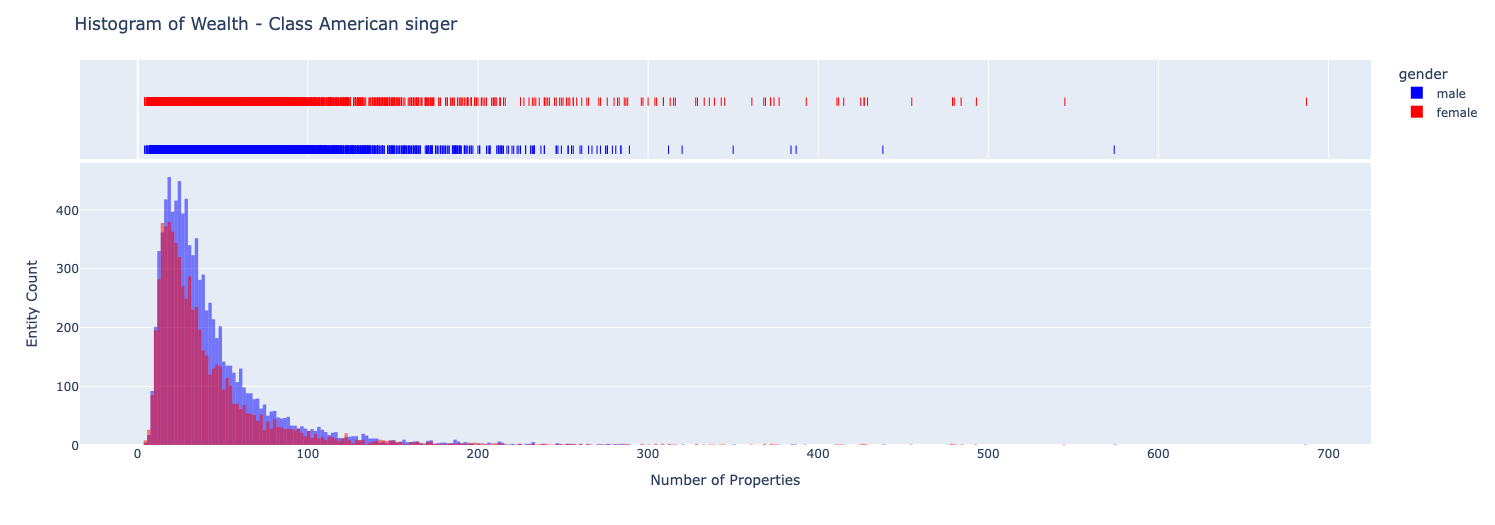
\includegraphics[clip,width=1.0\columnwidth]{Histogram of Wealth - American Singer}%
}

\caption{Histogram of wealth} \label{fig:Histogram of Wealth}

\end{figure}

At a glance we saw female classes are poorer compared to the male classes. To test this, we will use t-test and Welch's test. First, we performed F-test to check if the male and female classes have equal variance. The result of F-test is then used to determine the appropiate test to be used in each class. Those with equal variance will use t-test; otherwise Welch's test is used. Then, we performed the tests to verify the null and alternative hypotheses with significance level of \(\alpha=5\%\) as follows:

\(H_0\): The means of wealth of males and females in a particular class are equal

\(H_1\): The means of wealth of males and females in a particular class are not equal

\begin{center}
\small
\begin{threeparttable}
\caption{F-Test, T-Test, and Welch's Test Result of 10 Wikidata Classes}
\label{tab:gender - mean test}
\begin{tabular}{c | c c c c c c} 

\toprule
    Class Name & \CellWithForceBreak{F-Test \\ statistic} & \CellWithForceBreak{F-Test \\ p-value} & \CellWithForceBreak{T-Test \\ statistic} & \CellWithForceBreak{T-Test \\ p-value} & \CellWithForceBreak{Welch's Test \\ statistic} & \CellWithForceBreak{Welch's \\ p-value} \\ [0.5ex] 

\midrule
    American actress/actor & 0.86 & 0.00 & 5.85 & 4.97e-09 & 5.80 & 6.89e-09\\
    American journalist & 1.47 & 1.00 & 12.80 & 2.45e-37 & 13.75 & 1.01e-42 \\
    American politician & 1.00 & 0.55 & 6.86 & 6.90e-12 & 6.87 & 6.94e-12 \\
    American researcher & 1.91 & 1.00 & 6.43 & 1.35e-10 & 7.28 & 4.15e-13 \\
    American singer & 0.64 & 0.00 & 0.75 & 0.45 & 0.73 & 0.47 \\
    American writer & 1.73 & 1.00 & 24.80 & 1.56e-134 & 25.98 & 2.96e-147 \\
    Computer scientist & 1.75 & 1.00 & 5.43 & 5.57e-08 & 6.60 & 4.61e-11 \\
    Badminton player & 0.81 & 0.00 & -2.63 & 8.46e-03 & -2.62 & 8.86e-03 \\
    Businessperson & 0.53 & 0.00 & -4.48 & 7.56e-06 & -3.49 & 4.81e-04 \\
    Lawyer & 1.58 & 1.00 & 27.06 & 1.16e-160 & 32.16 & 8.04e-220 \\
    [1ex]

\bottomrule

\end{tabular}
\begin{tablenotes}
    \footnotesize
    \item{}
\end{tablenotes}
\end{threeparttable}
\end{center}

From the test results in \autoref{tab:gender - mean test}, we rejected the null hypothesis in 9 out of 10 class--American singer being the only exception. 7 out of 9 classes are in favor of male. The other 2 classes, American singer and . We concluded that female classes are more likely to have smaller means than male classes.

Here, a new measure is defined: top \(x\)\% male/female relative to the expectation. The value of expectation of a gender in a class is equal to the percentage of that particular in the class. Top \(x\)\% male relative to expectation is the ratio of percentage of male entities in the top \(x\)\% to the expectation. Similarly, top \(x\)\% female relative to expectation is the ratio of percentage of female entities in the top \(x\)\% to the expectation.

When the shape of distribution of male and female of a class is the same (in other word, the wealth is distributed equivalently to male and female entities), then the value of top \(x\)\% relative to expectation should be 1 for both male and female subclasses. A value higher than 1 indicates domination by that particular gender.

\begin{figure}[htp]
\centering 
\subfloat[Ratio of Class Wealth to Expectation per Cumulative Top Percentage - All Classes Average
\label{fig:test1}]{%
  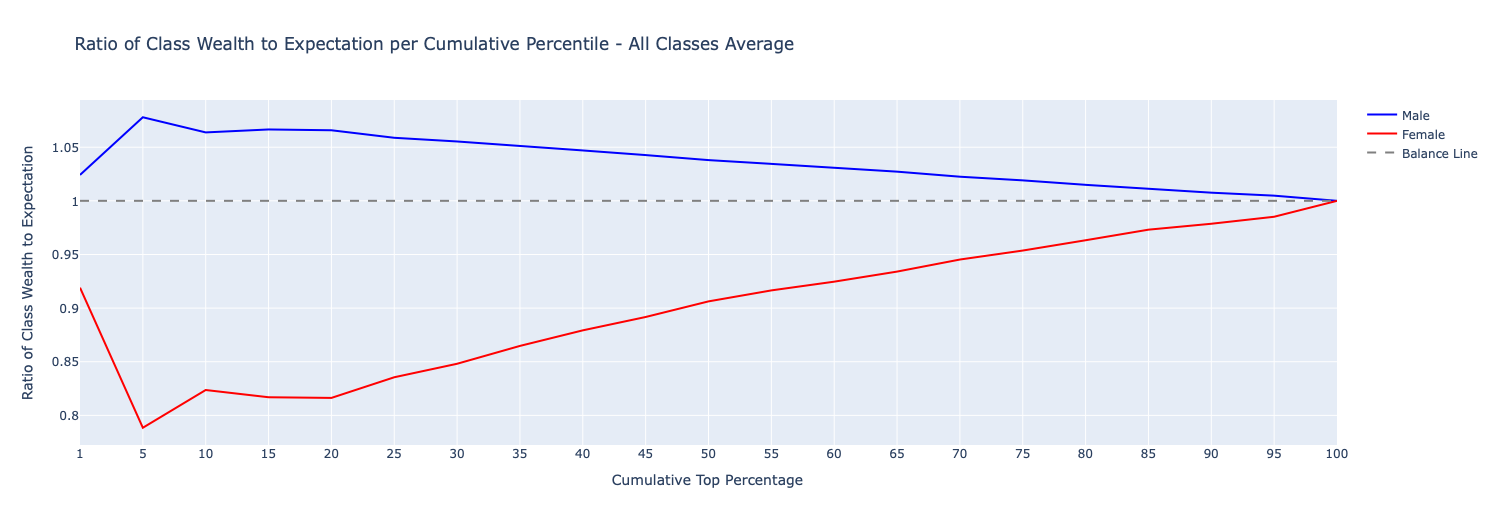
\includegraphics[clip,width=1.0\columnwidth]{Ratio of Class Wealth to Expectation per Cumulative Top Percentage - All Classes Average - Gender}%
}

\subfloat[Ratio of Class Wealth to Expectation per Quantile - All Classes Average\label{fig:test2}]{%
  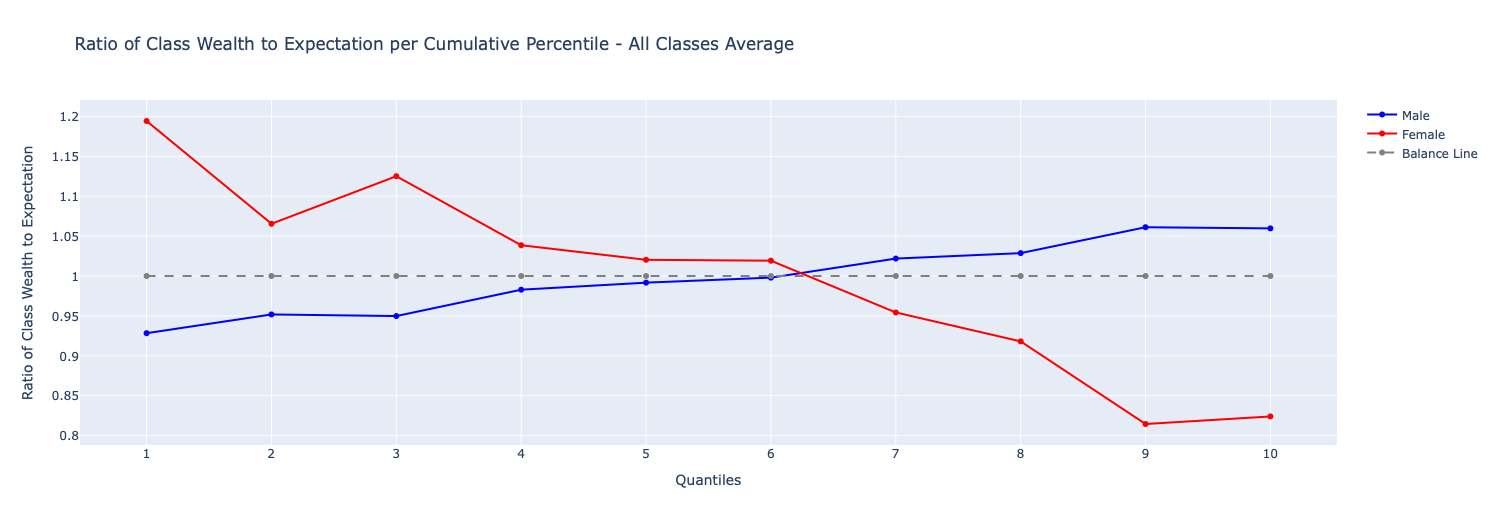
\includegraphics[clip,width=1.0\columnwidth]{Ratio of Class Wealth to Expectation per Quantile - All Classes Average - Gender}%
}

\caption{Ratio of each gender wealth to expectaion} \label{fig:gender - ratio of gender wealth to expectation}

\end{figure}

From \autoref{fig:gender - ratio of gender wealth to expectation} the value of ratio between top \(x\)\% potion to the expectation in the above tables, we can see that on average, the rich entities are dominated by male. Exceptions are held for 3 classes, that is classes American singer, businessperson, and badminton player. Moreover, as we set bigger portions (higher percentage), the gap of ratio between the two ender in each class decreases i.e. the value of top \(x\)\% relative to expectation of both genders converge to 1.
% \paragraph{Western Bias in Wikidata.}
\paragraph{Regional Knowledge Gap: Western vs. Non-Western Representation.}
Regional knowledge gap analysis in Wikidata will be performed on 5 Wikidata classes: computer scientist, singer, memorial, university, and river. For each class, we collected the data for the western portion from 8 countries: Canada, France, Germany, Ireland, Poland, Switzerland, the United Kingdom (UK), and the United State of America (USA). For the non-western portion, we also selected 8 countries: China, Egypt, India, Indonesia, Japan, Morocco, Nigeria, and South Africa. The selected countries represent different continents to capture a diverse geographic distribution. Additionally, we focused on large and well-known countries to ensure the dataset is representative, as data from smaller countries may not provide meaningful insights due to limited coverage in Wikidata.

To analyze the gap, the first aspect that will be considered is the proportion of each regional category in every class. We assumed that there are equal numbers of western and non-western and this will be the basis to determine if there is any gap in the data. Pearson's chi-square test (goodness-of-fit) is then performed to test the null and alternative hypotheses with significance level of \(\alpha=5\%\) as follows:

% \(H_0\): The proportions of western and non-western entities in a particular class are equal

% \(H_1\): The proportions of western and non-western entities in a particular class are not equal

\begin{table}[h]
    \centering
    \renewcommand{\arraystretch}{1.3}
    \begin{tabular}{|l p{12cm}|} 
        \hline
        \multicolumn{2}{|l|}{\textbf{Regional Knowledge Gap: Entity Count Gap (Pearson's chi-square test)}} \\
        \hline
        \textbf{$H_0$} & The proportions of western and non-western entities in a particular class are equal. \\
        \textbf{$H_1$} & The proportions of western and non-western entities in a particular class are not equal. \\
        \hline
        \textbf{Insight 1:} & Across all 5 classes, the proportions of western and non-western entities differ significantly. Western entities dominate in 4 out of 5 classes, with the only exception being the university class, which is skewed toward non-western entities. \\
        \hline
    \end{tabular}
\end{table}

% \vspace{-3em}

\begin{center}
\scriptsize
\begin{threeparttable}
\captionsetup{font=small}
\caption{Entity Count of 5 Wikidata Classes per Regional Category}
\label{tab:western - entity count}
\begin{tabular}{c | c c c c c c c} 

\toprule
    Class Name & Entity & Western & \CellWithForceBreak{Non- \\ western} & \%Western & \CellWithForceBreak{\%Non- \\ western}& $\chi^2$ & p-value \\ [0.5ex] 
\midrule
    Computer scientist & 6063 & 5446 & 617 & 0.90 & 0.10 & 3846.15 & 0.0 \\
    Singer & 43240 & 31039 & 12201 & 0.72 & 0.28 & 8206.99 & 0.0 \\
    Memorial & 4011 & 3836 & 175 & 0.96 & 0.04 & 3341.54 & 0.0 \\
    University & 6124 & 2398 & 3726 & 0.39 & 0.61 & 287.98 & 1.37e-64 \\
    River & 125567 & 70059 & 55508 & 0.56 & 0.44 & 1686.20 & 0.0 \\
    [1ex]
\bottomrule
\end{tabular}
\begin{tablenotes}
    \scriptsize
    \item{This table shows the entity count of 5 Wikidata classes per regional category. Chi-square test result shows the significance of difference between the entity count of the two regions.}
\end{tablenotes}
\end{threeparttable}
\end{center}

From \autoref{tab:western - entity count}, we can observe that the proportion of western entities exceeds that of non-western entities in 4 out of the 5 classes. In the memorial and computer scientist classes, the gap is particularly striking, with western entities making up over 90\% of the total population. Similarly, in the singer and river classes, western entities also represent the majority. The university class is the only exception, where non-western entities slightly outnumber western ones, comprising 61\% of the total. Based on the results of the chi-square test, the p-values in all five classes are well below the significance threshold ($\alpha = 0.05$), leading us to reject the null hypothesis. This indicates that the differences in entity proportions between western and non-western entities are statistically significant and not due to random variation.

However, similar to entity count in gender-based knowledg gap analysis, it is debatable that some of these gaps are expected. For instance, the dominance of western representation in the computer scientist or memorial classes is not necessarily a result of data entry errors or systemic bias within Wikidata alone. Instead, it may mirror general historical and sociopolitical factors, such as unequal access to documentation, global academic visibility, and archival infrastructure. Conversely, the university class, where the number of non-western entities are higher, might be a reflection of population-driven realities, as countries like China, India, and Indonesia possess massive populations and have established a vast number of higher education institutions to serve their demographic needs. The greater number of non-western universities represented in Wikidata is probably a result of this population scale. Due to this, raw entity count alone may not be an ideal measure of gap. To more accurately assess representation and equity, we must consider other metrics that analyze wealth distribution and prominence at the entity level.

% From \autoref{tab:western - central tendency}, non-western entities generally have lower values of measure of central tendency (mean, median, mode). The range of property count of non-westerns is generally also lower than the westerns. Positive values of skewness (skewness > 0) and high kurtosis values (kurtosis > 3) in all classes denote the wealth distribution is right skewed and leptokurtic.

The next step in our analysis is examining the measures of central tendency and dispersion to evaluate where the knowledge wealth is concentrated and how it varies between western and non-western entities.

\begin{table}[h]
    \centering
    \renewcommand{\arraystretch}{1.3}
    \begin{tabular}{|l p{12cm}|} 
        \hline
        \multicolumn{2}{|l|}{\textbf{Regional Knowledge Gap: Measures of Central Tendency and Dispersion}} \\
        \hline
        \textbf{Insight 1:} & In 4 out of 5 classes, western entities have higher mean, median, and mode values than non-western entities, indicating greater concentration of knowledge wealth. \\
        \textbf{Insight 2:} & Western entities generally exhibit higher standard deviations, skewness, and kurtosis, suggesting greater variability, more frequent outliers, and stronger right-skewed distributions. \\
        \hline
    \end{tabular}
\end{table}

% \vspace{-3em}

\begin{center}
\scriptsize
\begin{threeparttable}
\captionsetup{font=small}
\caption{Measures of Central Tendency of 5 Wikidata Classes per Regional Category}
\label{tab:western - central tendency}
\begin{tabular}{c | c c c} 
\toprule
    Class Name & \CellWithForceBreak{Mean \\ (o/w/n)} & \CellWithForceBreak{Median \\ (o/w/n)} & \CellWithForceBreak{Mode \\ (o/w/n)} \\ [0.5ex] 
\midrule
    Computer scientist & 35.00/35.87/27.24 & 29.00/29.00/22.00 & 21/15/16 \\
    Singer & 34.99/39.14/24.43 & 25.00/29.00/18.00 & 15/18/14 \\
    Memorial & 11.04/11.04/11.13 & 9.00/9.00/9.00 & 9/9/9 \\
    University & 23.11/31.61/17.63 & 17.50/24.00/16.00 & 6/6/6 \\
    River & 7.69/8.55/6.60 & 7.00/7.00/6.00 & 7/7/7 \\
    [1ex]
\bottomrule
\end{tabular}
\begin{tablenotes}
    \scriptsize
    \item{This table shows the measures of central tendency of 5 Wikidata classes per regional category. Each measure will have 3 values: o (overall), w (western), and n (non-western).}
\end{tablenotes}
\end{threeparttable}
\end{center}

% \vspace{-2em}

\begin{center}
\scriptsize
\begin{threeparttable}
\captionsetup{font=small}
\caption{Measures of Dispersion and Symmetry of 5 Wikidata Classes per Regional Category}
\label{tab:western - dispersion and symmetry}
\begin{tabular}{c | c c c c c} 

\toprule
    Class Name & \CellWithForceBreak{Min \\ (o/w/n)} & \CellWithForceBreak{Max \\ (o/w/n)} & \CellWithForceBreak{Std. Deviation \\ (o/w/n)} & \CellWithForceBreak{Skewness \\ (o/w/n)} & \CellWithForceBreak{Kurtosis \\ (o/w/n)} \\ [0.5ex] 
\midrule
    Computer scientist & 4/4/5 & 441/441/145 & 25.15/25.67/18.15 & 3.02/3.02/2.37 & 20.90/20.83/8.49 \\
    Singer & 3/4/3 & 687/687/379 & 33.27/36.60/18.94 & 4.49/4.28/3.15 & 35.56/31.09/21.59 \\
    Memorial & 2/3/2 & 142/142/52 & 5.89/5.82/7.28 & 8.50/8.95/2.98 & 143.57/156.15/12.79 \\
    University & 2/2/2 & 234/234/166 & 20.00/25.88/12.25 & 2.37/1.65/2.22 & 10.34/5.33/12.70 \\
    River & 2/2/2 & 452/452/148 & 5.24/6.46/2.68 & 21.71/19.54/14.67 & 1152.84/868.56/465.42 \\
    [1ex]
\bottomrule
\end{tabular}
\begin{tablenotes}
    \scriptsize
    \item{This table shows the measures of dispersion and symmetry of 5 Wikidata classes per regional category. Each measure will have 3 values: o (overall), w (western), and n (non-western).}
\end{tablenotes}
\end{threeparttable}
\end{center}

From \autoref{tab:western - central tendency}, we observed that in 4 out of 5 classes, western entities consistently show higher values across all measures of central tendency (mean, median, and mode) compared to non-western entities. This suggests that western entities tend to be richer in knowledge wealth. The memorial class is the only exception, where both groups exhibit nearly identical values. A particularly extreme disparity is observed in the university class, where the mean property count for western entities (31.61) is nearly double that of non-western entities (17.63), highlighting a strong central tendency skew. This extreme pattern can also be seen in the singer class.

Turning to the measures of dispersion and symmetry in \autoref{tab:western - dispersion and symmetry}, we saw that standard deviation is generally higher for western entities across all classes except memorial, suggesting greater wealth variability among western entities. Furthermore, in the university class, western entities show a standard deviation of 25.88, more than double that of non-western entities at 12.25. We also observed positive skewness and high kurtosis across all classes and both regions, indicating that knowledge wealth distributions are right-skewed and leptokurtic. However, western entities often exhibit higher values, implying more extreme outliers and longer tails. For example, in the river class, the skewness and kurtosis for western entities are 19.54 and 868.56, respectively, compared to 14.67 and 465.42 for non-western entities.

Taken together, these statistics suggest that western entities tend not only to accumulate more knowledge wealth on average but also to dominate the extreme high end of the distribution. In contrast, non-western entities tend to cluster around lower values with tighter distribution, reinforcing regional disparity in knowledge representation.

At a glance, western entities appear to be richer compared to their non-western counterparts. To statistically verify this, we conducted a series of mean comparison tests between the two groups. We began by applying the F-test to assess whether the western and non-western subsets within each class have equal variance. The result of the F-test determines the appropriate test to be used: if the p-value is greater than 0.05, indicating equal variance, we use the standard t-test; otherwise, we apply Welch's test, which does not assume equal variance.

% Out of 5 classes, class of memorial is the only class where the null hypothesis is not rejected. In the other 4 classes, we can see a significant difference between the mean of the two reginal categories, which all are in favor of the western.

\begin{table}[h!]
    \centering
    \renewcommand{\arraystretch}{1.3}
    \begin{tabular}{|l p{12cm}|} 
        \hline
        \multicolumn{2}{|l|}{\textbf{Regional Knowledge Gap: Mean of Wealth Gap (two-sided t-test and Welch's test)}} \\
        \hline
        \textbf{$H_0$} & The means of wealth of western and non-western entities in a particular class are equal. \\
        \textbf{$H_1$} & The means of wealth of western and non-western entities in a particular class are not equal. \\
        \hline
        \textbf{Insight 1:} & In 4 out of 5 classes, western entities have significantly higher mean knowledge wealth than non-western entities. \\
        \hline
    \end{tabular}
\end{table}

% \vspace{-3em}

\begin{center}
\scriptsize
\begin{threeparttable}
\captionsetup{font=small}
\caption{F-Test, T-Test, and Welch's Test Result of 5 Wikidata Classes}
\label{tab:western - mean test}
\begin{tabular}{c | c c c c c c} 
\toprule
    Class Name & \CellWithForceBreak{F-Test \\ statistic} & \CellWithForceBreak{F-Test \\ p-value} & \CellWithForceBreak{T-Test \\ statistic} & \CellWithForceBreak{T-Test \\ p-value} & \CellWithForceBreak{Welch's Test \\ statistic} & \CellWithForceBreak{Welch's \\ p-value} \\ [0.5ex] 
\midrule
    Computer scientist & 2.00 & 1.00 & 8.13 & 5.10e-16 & - & - \\
    Singer & 3.73 & 1.00 & 42.22 & 0.0 & - & - \\
    Memorial & 0.64 & 0.00 & - & - & -0.16 & 0.88 \\
    University & 4.46 & 1.00 & 28.40 & 8.23e-167 & - & - \\
    River & 5.83 & 1.00 & 66.91 & 0.0 & - & - \\
 [1ex]
\bottomrule
\end{tabular}
\begin{tablenotes}
    \scriptsize
    \item{}
\end{tablenotes}
\end{threeparttable}
\end{center}

The result of the F-test in \autoref{tab:western - mean test} shows that only one class, that is, memorial, has unequal variance (p < 0.05), thus requiring the use of Welch's test. For the remaining four classes, the t-test was applied. From the test results, we rejected the null hypothesis in 4 out of 5 classes, indicating that the difference in mean wealth between western and non-western entities is statistically significant. The only exception is the memorial class, where Welch's test yields a p-value of 0.88, suggesting no significant difference in mean. Among the classes with significant results, the direction of difference consistently favors Western entities. This can be seen clearly in classes such as university and singer, where the t-statistics are noticeably high (28.40 and 42.22, respectively) and the p-values are zero. These findings align with our previous observations that western entities dominate in terms of quantity and average information richness. We conclude that western entities are more likely to have higher mean knowledge wealth than non-western ones, although exceptions like the memorial class suggest that certain domains may present a more balanced knowledge distribution.

As with gender-based knowledge gap, measuring regional gap in Wikidata cannot rely solely on entity counts. The number of entities associated with western and non-western regions may reflect real-world disparities in documentation or notability, making raw counts an unreliable indicator of gap. Similarly, measures of central tendency, such as the mean or median, fail to capture how representation is distributed across the full spectrum of prominence or wealth. To address these limitations, we applied the same metric introduced in the gender-based gap analysis: the relative expectation ratio. This measure compares a region's share of entities within a given quantile to its expected share under equal representation. A ratio of 1 indicates proportional representation, while values above or below 1 signal overrepresentation or underrepresentation, respectively. This allows for a more nuanced, quantile-level understanding of how western and non-western entities are distributed in knowledge graphs like Wikidata.

\begin{table}[h]
    \centering
    \renewcommand{\arraystretch}{1.3}
    \begin{tabular}{|l p{12cm}|} 
        \hline
        \multicolumn{2}{|l|}{\textbf{Regional Knowledge Gap: Relative Expectation Ratios}} \\
        \hline
        \textbf{Insight 1:} & On average across all 5 classes, the less prominent segments are dominated by non-western entities, while the more prominent ones are dominated by western entities. The middle quantiles exhibit a zig-zag pattern, reflecting inconsistent representation between the two groups. \\
        \textbf{Insight 2:} & At the individual class level, 2 out of 5 classes display a particularly strong western dominance. The rests exhibit a zig-zag trend. \\
        \hline
    \end{tabular}
\end{table}

On average across all classes, the lower four quantiles (i.e., the less prominent or "poorer" segments) are predominantly composed of non-western entities, while the top three quantiles (i.e., the more prominent or "wealthier" segments) are dominated by western entities. The middle quantiles exhibit a zig-zag pattern, reflecting inconsistent representation between the two groups. At the individual class level, the computer scientist and singer classes display a particularly strong western bias. In both classes, non-western entities are consistently overrepresented in the lower quantiles (Q1–Q4), while western entities are consistently overrepresented in the upper quantiles (Q5–Q6). This pattern suggests a clear stratification, with non-western entities disproportionately concentrated in less prominent positions. The memorial, university, and river classes, however, deviate from this pattern and exhibit a zig-zag trend across quantiles. This suggests a more unstable distribution of western and non-western entities across the quantiles.

\begin{figure}
\centering 
\subfloat[Ratio of Class Wealth to Expectation per Cumulative Top Percentage - All Classes Average
\label{fig:test1 - western}]{%
  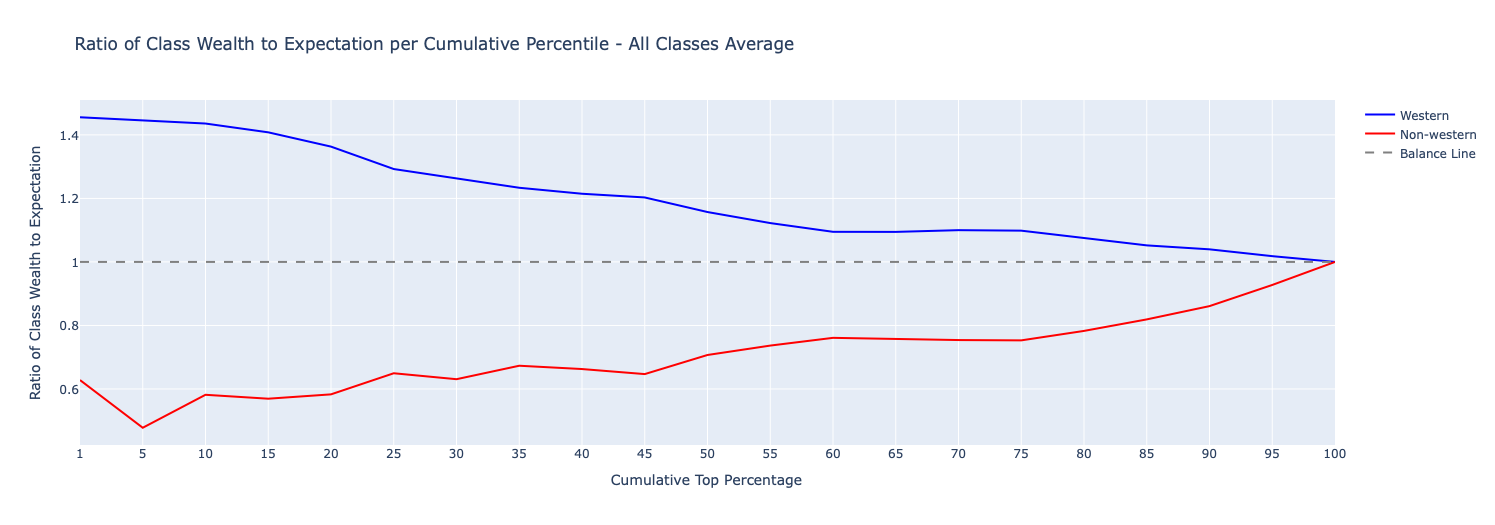
\includegraphics[clip,width=1.0\columnwidth]{Ratio of Class Wealth to Expectation per Cumulative Top Percentage - All Classes Average - Region}%
}

\subfloat[Ratio of Class Wealth to Expectation per Quantile - All Classes Average\label{fig:test2 - western}]{%
  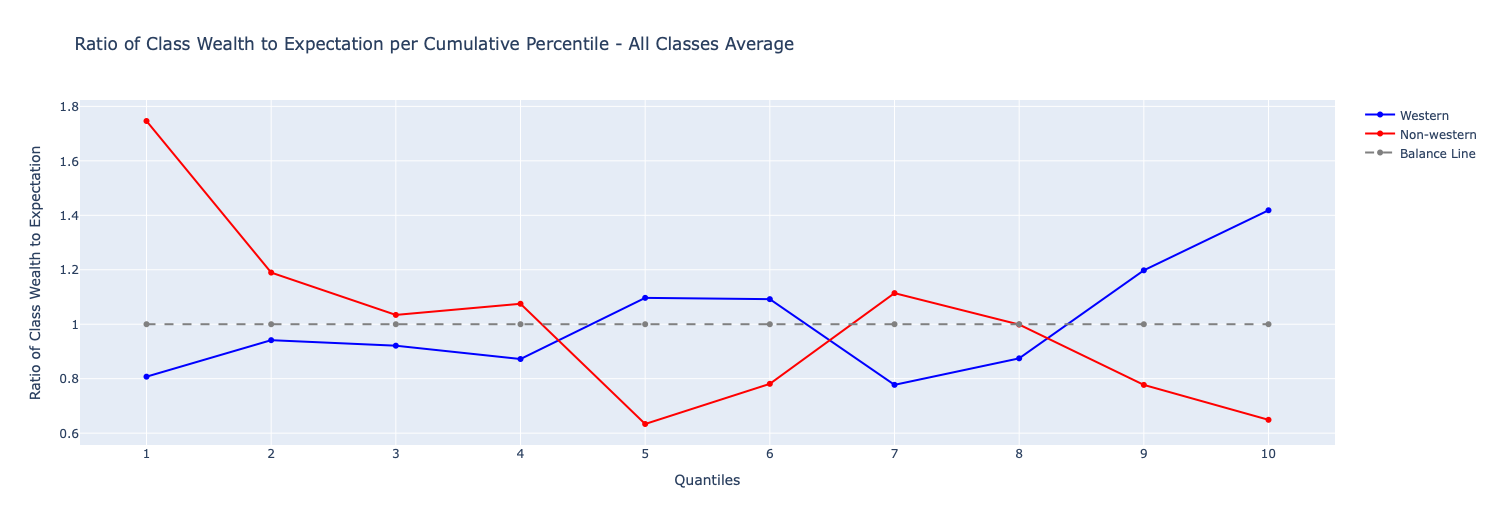
\includegraphics[clip,width=1.0\columnwidth]{Ratio of Class Wealth to Expectation per Quantile - All Classes Average - Gender - Region}%
}

\caption{Ratio of each regional wealth to expectation}\label{fig:western - ratio of regional wealth to expectation}

\end{figure}
\subsection{Effect of Type of Wealth on Inequality Measure} \label{wealth & gini}

% \begin{center}
    \small
    \begin{threeparttable}
    \caption{Gini Bag-Set}
    \label{tab:gini bag-set}
    \begin{tabular}{c c c} 
    
    \toprule
        Class Name & Gini Bag & Gini Set \\ [0.5ex] 
    \midrule
        Historical painting & 0.22 & 0.14 \\
        University & 0.44 & 0.41 \\
        Sci-fi book & 0.32 & 0.22 \\
        Memorial & 0.22 & 0.18 \\
        American researcher & 0.33 & 0.31 \\
        American singer & 0.40 & 0.39 \\
        Badminton player & 0.29 & 0.14 \\
        Computer scientist & 0.41 & 0.37 \\
        [1ex]
    \bottomrule
    \end{tabular}
    \begin{tablenotes}
        \footnotesize
        This table shows the measures of gini coefficient of knowledge wealth based on the (non-)uniqueness of individual properties of 8 Wikidata classes
    \end{tablenotes}
    \end{threeparttable}
\end{center}
% \begin{center}
    \small
    \begin{threeparttable}
    \caption{Gini Object-Literal-ID}
    \label{tab:gini proptype}
    \begin{tabular}{c c c c} 
    
    \toprule
        Class Name & Gini Object & Gini Literal & Gini ID \\ [0.5ex] 
    \midrule
        American researcher & 0.26 & 0.50 & 0.50 \\
        American singer & 0.29 & 0.50 & 0.53 \\
        Badminton player & 0.30 & 0.36 & 0.60 \\
        Computer scientist & 0.36 & 0.54 & 0.56 \\
        Historical painting & 0.25 & 0.27 & 0.44 \\
        Memorial & 0.20 & 0.30 & 0.40 \\
        Sci-fi book & 0.35 & 0.34 & 0.42 \\
        University & 0.40 & 0.49 & 0.53 \\
        [1ex]
    \bottomrule
    \end{tabular}
    \begin{tablenotes}
        \footnotesize
        This table shows the measures of gini coefficient of knowledge wealth based on types of property of 8 Wikidata classes
    \end{tablenotes}
    \end{threeparttable}
\end{center}
% \begin{center}
    \small
    \begin{threeparttable}
    \caption{Gini Outgoing-Incoming}
    \label{tab:gini outgoing-incoming}
    \begin{tabular}{c c c} 
    
    \toprule
        Class Name & Gini Outgoing & Gini Incoming \\ [0.5ex] 
    \midrule
        Historical painting & 0.22 & 0.86 \\
        University & 0.44 & 0.91 \\
        Sci-fi book & 0.32 & 0.82 \\
        Memorial & 0.22 & 0.99 \\
        American researcher & 0.33 & 0.77 \\
        American singer & 0.40 & 0.82 \\
        Badminton player & 0.29 & 0.68 \\
        Computer scientist & 0.41 & 0.81 \\
        [1ex]
    \bottomrule
    \end{tabular}
    \begin{tablenotes}
        \footnotesize
        This table shows the measures of gini coefficient of knowledge wealth based on the direction of link of 8 Wikidata classes
    \end{tablenotes}
    \end{threeparttable}
\end{center}

In this subchapter, analysis is done to see how each wealth type affects the level of inequality of Wikidata classes. There are 2 ways this is done--quantitatively using Gini coefficient and qualitatively using Lorenz curve. The analysis is performed on 8 Wikidata classes, in which 4 of them are human-related class while the other 4 are not.

When looking at the notion of wealth using the characteristics of (non-)uniqueness of individual properties, it is intuitive that the measure of bag of properties will always give higher (or at least, equal) amount of wealth compared to the measure of set. Set of property will have an upper bound of number of unique property, while bag of properties does not have any upper bound. Moreover, using bag of properties, a large number of triples having the same property may inflate the wealth substantially--though this is not necessarily a problem nor an advantage. This characteristics has a direct impact on inequality measure and it is well depicted on the value of Gini coefficient. From \autoref{table:gini-coef}, in all clasess, the Gini coefficient using bag of properties is always higher than of set of properties.

% - object, literal, ID: object tends to have lower inequality
Using the notion of wealth by type of property, in general the smallest Gini coefficient value is mostly from wealth using object property. The second one is when using literal, while the biggest one always comes when using ID.

% - outgoing, incoming: incoming shows very high Gini, this is because it is harder --> show the lorenz curve
Using the notion of wealth by the direction of the link, the Gini coefficient when using incoming link is always higher than using outgoing link. By inspecting the Lorenz curve, we can see that most entities do not have any incoming link, and only the small percentage of entites has some incoming link. \autoref{fig:gini-outgoin&incoming} shows the comparison of Lorenz curve of knowledge wealth based on the direction of the link from 3 Wikidata classes. The difference between the two is very significant, because in \autoref{fig:gini-outgoing} the Lorenz curves are closer to the perfect equality line, meanwhile in \autoref{fig:gini-incoming} the diagonal and the Lorenz curve almost form a right triangle which is very close to maximum inequality.

% add to discussion 
% - Wikidata = entity-centric knowledge graph, dimana bentuknya (s,p,o) dengan s sebagai subject of interest. jadi memang expected bahwa outgoing banyak 
% sedangkan incoming mostly justru 0.
% - sedrastis ini perbedaan incoming vs outgoing. incoming link is underestimated. given o, what is the (s, p)
% - kasih contoh: 2 entitas yang secara outgoing mirip, tapi incoming-nya jomplang (1 kaya 1 miskin)

\begin{center}
    \small
    \begin{threeparttable}
    \caption{Knowledge Wealth Type on Gini Coefficient}
    \label{table:gini-coef}
    \begin{tabular}{c | c c | c c c | c c} 
    
    \toprule
        Class Name & \CellWithForceBreak{Gini \\ Bag} & \CellWithForceBreak{Gini \\ Set} & \CellWithForceBreak{Gini \\ Object} & \CellWithForceBreak{Gini \\ Literal} & \CellWithForceBreak{Gini \\ ID} & \CellWithForceBreak{Gini \\ Outgoing} & \CellWithForceBreak{Gini \\ Incoming} \\ [0.5ex] 
    \midrule
        American researcher & 0.33 & 0.31 & 0.25 & 0.27 & 0.44 & 0.33 & 0.77 \\
        American singer & 0.40 & 0.39 & 0.20 & 0.30 & 0.40 & 0.40 & 0.82 \\
        Badminton player & 0.29 & 0.14 & 0.35 & 0.34 & 0.42 & 0.29 & 0.68 \\
        Computer scientist & 0.41 & 0.37 & 0.40 & 0.49 & 0.53 & 0.41 & 0.81 \\
        Memorial & 0.22 & 0.18 & 0.36 & 0.54 & 0.56 & 0.22 & 0.99 \\
        Historical painting & 0.22 & 0.14 & 0.26 & 0.50 & 0.50 & 0.22 & 0.86 \\
        Sci-fi book & 0.32 & 0.22 & 0.30 & 0.36 & 0.60 & 0.32 & 0.82 \\
        University & 0.44 & 0.41 & 0.29 & 0.50 & 0.53 & 0.44 & 0.91 \\
        [1ex]
    \bottomrule
    \end{tabular}
    \begin{tablenotes}
        \footnotesize
        \item{This table shows the comparison of Gini coefficient of 8 Wikidata classes}
    \end{tablenotes}
    \end{threeparttable}
\end{center}

\begin{figure}[!h]
    \centering 
    \subfloat[Lorenz curve of wealth using outgoing link
    \label{fig:gini-outgoing}]{%
      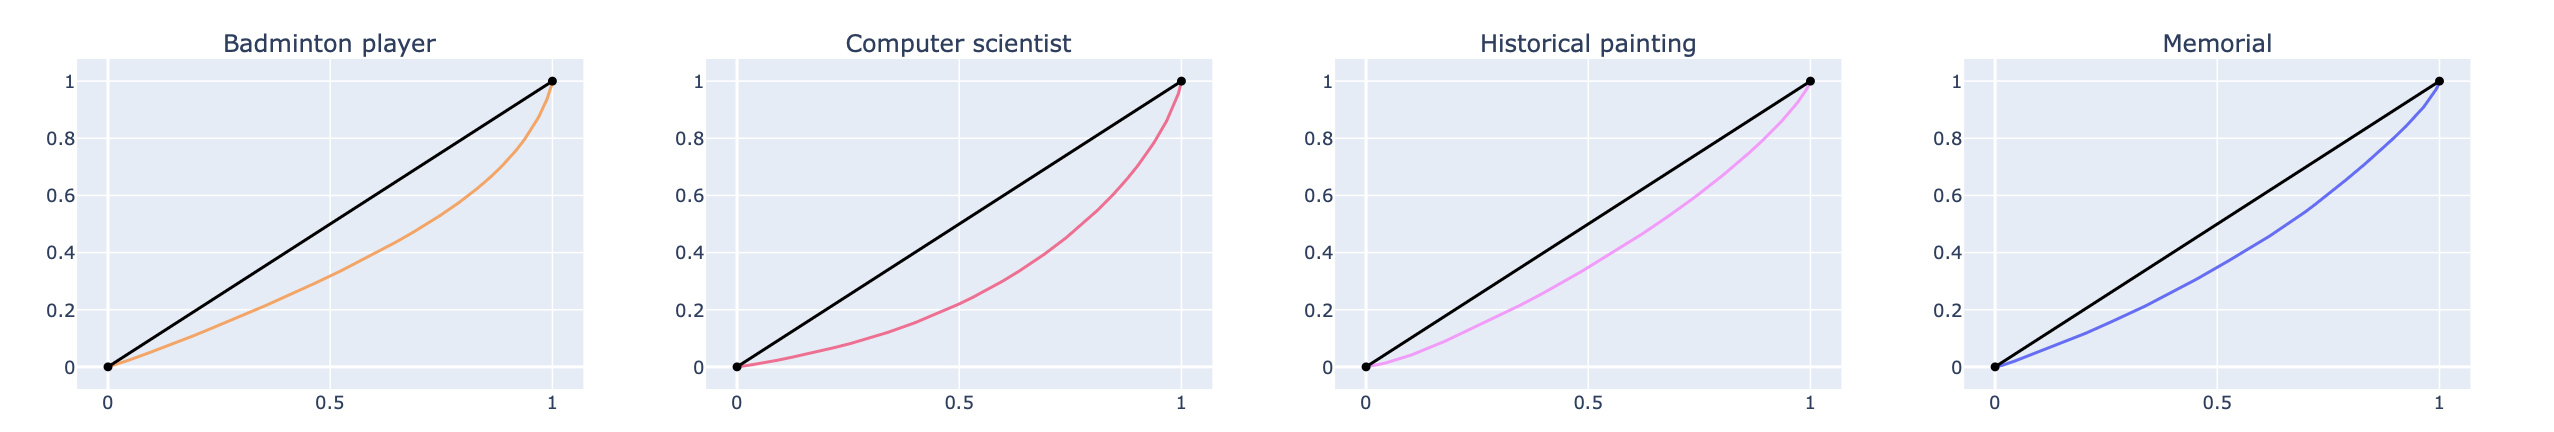
\includegraphics[clip,width=1.0\columnwidth]{Gini - Outgoing}%
    }
    
    \subfloat[Lorenz curve of wealth using incoming link\label{fig:gini-incoming}]{%
      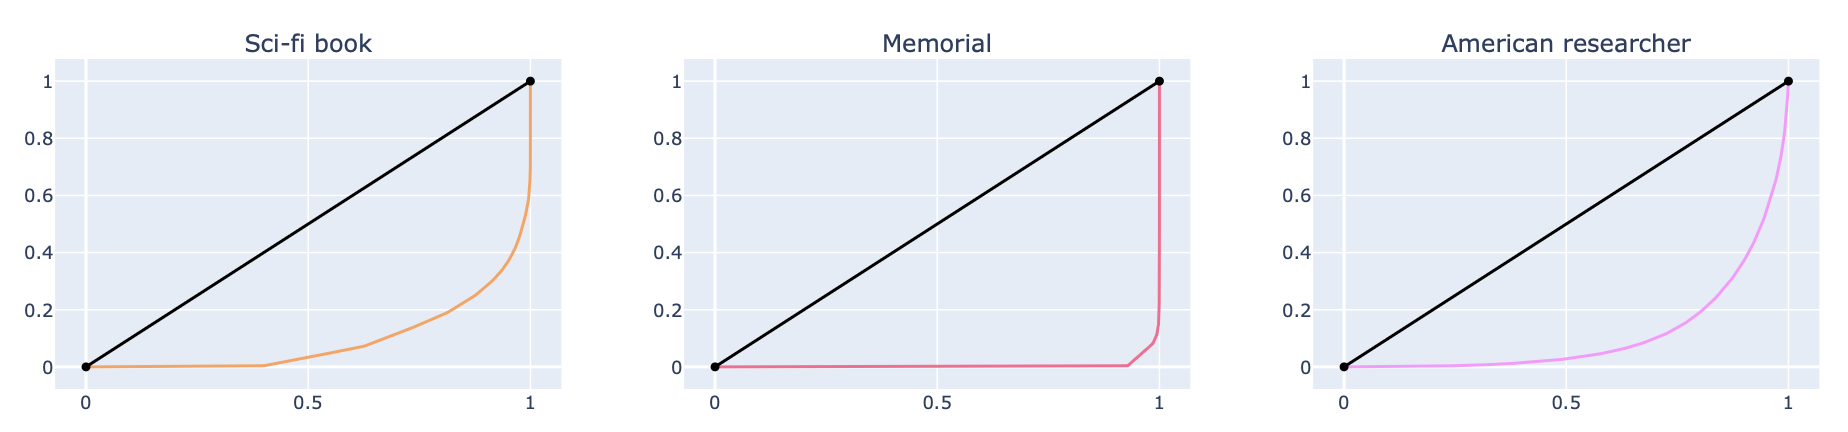
\includegraphics[clip,width=1.0\columnwidth]{Gini - Incoming.png}%
    }
    
    \caption{Comparison of Lorenz curve of wealth based on the direction of link} \label{fig:gini-outgoin&incoming}
    
\end{figure}
\subsection{Contribution of Property Type to Knowledge Wealth} \label{wealth & proptype contribution}

In this subchapter, analysis is done to see how much contribution of each property types to the knowledge wealth of Wikidata classes. The analysis is performed on 8 Wikidata classes, in which 4 of them are human-related class while the other 4 are not. The wealth of each classes is calculated using the concept of bag of properties and set of properties, for each property types (object, literal, ID, and their combinations).

Two methods of averaging are used in this analysis—global percentage and average contribution per individual entity. The first method is done by calculating the total sum of each property across all entities and then dividing it by the grand total of all properties combined, providing a holistic view of each property's overall contribution. The second method is done by first determining the percentage contribution of each property within each individual entity and then averaging these percentages across all entities, ensuring that every entity is equally represented regardless of its scale. While the global percentage method highlights absolute contributions, the average per-entity method captures relative contributions within each entity, making it more robust to variations in scale.

\begin{center}
    \small
    \makebox[\linewidth]{
    \begin{threeparttable}
    \caption{Contribution of Property Type to Knowledge Wealth Using Bag of Properties}
    \label{table:prop-contribution-bag}
    \begin{tabular}{c | c c c | c | c} 
    
    \toprule
        Class Name & \CellWithForceBreak{\% Object \\ Bag} & \CellWithForceBreak{\% Literal \\ Bag} & \CellWithForceBreak{\% ID \\ Bag} & \CellWithForceBreak{\% Literal + ID \\ Bag} & \CellWithForceBreak{\% Object + Literal \\ Bag} \\ [0.5ex] 
    \midrule
        American researcher & 59.55 / 65.65 & 3.32 / 2.8 & 37.12 / 31.55 & 40.45 / 34.35 & 62.88 / 68.45 \\
        American singer & 40.44 / 48.42 & 7.47 / 8.48 & 52.09 / 43.1 & 59.56 / 51.58 & 47.91 / 56.9 \\
        Badminton player & 79.34 / 78.96 & 10.14 / 11.68 & 10.52 / 9.36 & 20.66 / 21.04 & 89.48 / 90.64 \\
        Computer scientist & 59.36 / 65.93 & 4.19 / 3.71 & 36.44 / 30.36 & 40.64 / 34.07 & 63.56 / 69.64 \\
        Historical painting & 66.35 / 66.46 & 25.48 / 25.85 & 8.17 / 7.69 & 33.65 / 33.54 & 91.83 / 92.31 \\
        Memorial & 62.82 / 64.16 & 21.0 / 20.4 & 16.18 / 15.44 & 37.18 / 35.84 & 83.82 / 84.56 \\
        Sci-fi book & 62.96 / 62.62 & 14.44 / 15.78 & 22.59 / 21.6 & 37.04 / 37.38 & 77.41 / 78.4 \\
        University & 37.59 / 44.79 & 18.11 / 18.31 & 44.3 / 36.9 & 62.41 / 55.21 & 55.7 / 63.1 \\
        [1ex]
    \bottomrule
    \end{tabular}
    \begin{tablenotes}
        \footnotesize
        \item{This table shows the contribution of each property type of 8 Wikidata classes based on the notion of bag of properties. Each record has 2 values separated by "/". The first value is the contribution rate when calculated with global percentage method, and the second one is when using the average contribution per individual entity}
    \end{tablenotes}
    \end{threeparttable}
    }
\end{center}

\begin{center}
    \small
    \makebox[\linewidth]{
    \begin{threeparttable}
    \caption{Contribution of Property Type to Knowledge Wealth Using Set of Properties}
    \label{table:prop-contribution-set}
    \begin{tabular}{c | c c c | c | c} 
    
    \toprule
        Class Name & \CellWithForceBreak{\% Object \\ Set} & \CellWithForceBreak{\% Literal \\ Set} & \CellWithForceBreak{\% ID \\ Set} & \CellWithForceBreak{\% Literal + ID \\ Set} & \CellWithForceBreak{\% Object + Literal \\ Set} \\ [0.5ex] 
    \midrule
        American researcher & 51.25 / 59.69 & 3.97 / 3.29 & 44.78 / 37.02 & 48.75 / 40.31 & 55.22 / 62.98 \\
        American singer & 33.91 / 43.58 & 8.1 / 9.18 & 57.99 / 47.24 & 66.09 / 56.42 & 42.01 / 52.76 \\
        Badminton player & 71.75 / 74.13 & 13.79 / 13.9 & 14.46 / 11.97 & 28.25 / 25.87 & 85.54 / 88.03 \\
        Computer scientist & 50.53 / 60.54 & 4.98 / 4.27 & 44.49 / 35.19 & 49.47 / 39.46 & 55.51 / 64.81 \\
        Historical painting & 60.57 / 61.91 & 28.88 / 28.61 & 10.55 / 9.48 & 39.43 / 38.09 & 89.45 / 90.52 \\
        Memorial & 60.06 / 62.01 & 22.41 / 21.59 & 17.54 / 16.4 & 39.94 / 37.99 & 82.46 / 83.6 \\
        Sci-fi book & 59.36 / 61.91 & 13.86 / 14.59 & 26.78 / 23.5 & 40.64 / 38.09 & 73.22 / 76.5 \\
        University & 33.93 / 42.74 & 17.67 / 18.32 & 48.4 / 38.95 & 66.07 / 57.26 & 51.6 / 61.05 \\
        [1ex]
    \bottomrule
    \end{tabular}
    \begin{tablenotes}
        \footnotesize
        \item{This table shows the contribution of each property type of 8 Wikidata classes based on the notion of set of properties. Each record has 2 values separated by "/". The first value is the contribution rate when calculated with global percentage method, and the second one is when using the average contribution per individual entity}
    \end{tablenotes}
    \end{threeparttable}
    }
\end{center}

From \autoref{table:gini-coef} 
When we look at the contribution of each type of property to the overall wealth, ....
Overall, the usage of pure literal properties is lower than of object and ID. This aligns with the principle of knowledge graph to use URI for internal connections and ID for external resources.


% \subsection{(Tentative)Proxy of Knowledge Wealth: Real-World Rankings}
% - Popularity
% - Movie IMDb
% - GDP, economic wealth
% - Personal net worth

% \subsection{(Tentative) Basics of Knowledge Wealth Comparison}

% \paragraph{Subclass-to-Subclass Wealth Comparison}
% \paragraph{Subclass-to-Superclass Wealth Comparison}
% \paragraph{Totally Different Classes Wealth Comparison}

% \subsection{(Tentative) Knowledge Wealth Evolution using Wikidata History}

% \subsection{(Tentative) Pareto Principle in Wikidata}

% \subsection{(Tentative)}
% This is additional, if possible. Based on WN notes to use statistical measures for machine learning